%
% Complete documentation on the extended LaTeX markup used for Insight
% documentation is available in ``Documenting Insight'', which is part
% of the standard documentation for Insight.  It may be found online
% at:
%
%     http://www.itk.org/

\documentclass{InsightArticle}


%%%%%%%%%%%%%%%%%%%%%%%%%%%%%%%%%%%%%%%%%%%%%%%%%%%%%%%%%%%%%%%%%%
%
%  hyperref should be the last package to be loaded.
%
%%%%%%%%%%%%%%%%%%%%%%%%%%%%%%%%%%%%%%%%%%%%%%%%%%%%%%%%%%%%%%%%%%
\usepackage[dvips,
bookmarks,
bookmarksopen,
backref,
colorlinks,linkcolor={blue},citecolor={blue},urlcolor={blue},
]{hyperref}
% to be able to use options in graphics
\usepackage{graphicx}
% for pseudo code
\usepackage{listings}
% subfigures
\usepackage{subfigure}


%  This is a template for Papers to the Insight Journal. 
%  It is comparable to a technical report format.

% The title should be descriptive enough for people to be able to find
% the relevant document. 
\title{Label object representation and manipulation with ITK}

% Increment the release number whenever significant changes are made.
% The author and/or editor can define 'significant' however they like.
%\release{0.00}

% At minimum, give your name and an email address.  You can include a
% snail-mail address if you like.
\author{Ga\"etan Lehmann{$^1$}}
\authoraddress{{$^1$}INRA, UMR 1198; ENVA; CNRS, FRE 2857, Biologie du
D\'eveloppement et 
Reproduction, Jouy en Josas, F-78350, France.}

\begin{document}
\maketitle

\ifhtml
\chapter*{Front Matter\label{front}}
\fi


\begin{abstract}
\noindent

Richard Beare has recently introduced a new filter to efficiently labelize the
connected components with ITK, and has also proposed to use the {\em run-length
encoding} used in that filter to implement some of the most useful binary
mathematical morphology operators: the opening by attribute.
Following that idea, and after have searched a way to use the ITK's spatial
objects for this task, a new set of classes have been developed to represent and
manipulate the label images and the objects within them in ITK.
Those new classes have been used to implement several label images
manipulation based on object attributes, as well as the binary and label specialization of
some mathematical morphology filters based on the morphological reconstruction. This contribution comes
with 65 new classes, and should greatly enhance the binary mathematical
morphology in ITK.

All the source codes are provided, as well as a full set of tests and several
usage examples of the new classes.

\end{abstract}

\tableofcontents

\section{Introduction}

Identifying the objects in an image is a very common task, often realized by
producing an image of the same size with a single pixel value per object. This
image is called a label image. There are several way to create such image. It
can be done by searching the connected components in a binary image, it can be
produced directly by some algorithms, like the watershed transform, it can even
be simply done by hand, etc.

\section{Definitions}

In that article, some terms will be cited very frequently. I will try to define
them, in the context of the image analysis.

\subsection{Label}

A label is an identifier of something with the same caracteristics in the image.
Those caracteristics can be whatever you want, for example, the range of pixel
values, the same object in sense of connected component, etc.
A label can be represented by anything and only need to be unique in the image.
It doesn't even require to be ordered. In practice, we choose to use the
integral number types, for several reasons: they are commonly used in image
analysis, they efficiently reprensent the label in memory, and its easy to find
the next label by adding 1.

\subsection{Label image}

A label image is an image which contains several label pixels. Often, the
labels are representing some objects placed on a background, and so the label
image may use a particular label for the background.

\begin{figure}[htbp]
\begin{center}
\subfigure[A label Image.]{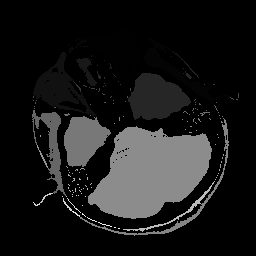
\includegraphics[scale=0.7]{cthead1-label2}}
\subfigure[The same image with colored labels]{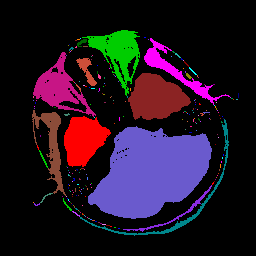
\includegraphics[scale=.7]{cthead1-label2-rgb}}
\caption{(a) the label image of connected components in Figure~\ref{fig:binaryImage}. (b) is the same image with labels colored with {\em itk::LabelToRGBImageFilter}.\label{fig:labelImage}}
\end{center}
\end{figure}

\subsection{Binary image}

A binary image is an image with two labels: a foreground label and a background
label. In practice, the binary images are using a pixel type able to store more
than those two values. The foreground is thus defined with a particular label,
and the other label in the image are considered as the background. A side effect
of that is that a label image can be considered as a binary image, and so, it
let us manipulate a single object in a label image.

\begin{figure}[htbp]
\begin{center}
\subfigure[A simple binary image.]{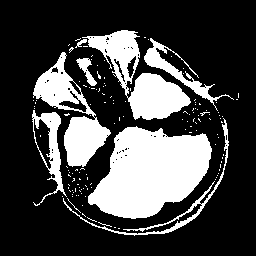
\includegraphics[scale=0.7]{cthead1-bin}}
\subfigure[A binary image, or a label image?]{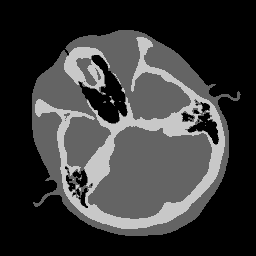
\includegraphics[scale=.7]{2th_cthead1}}
\caption{(a) is a simple binary image. Usually, the white pixel have the value 255, and the background the value 0. (b) contains 3 values (0, 100 and 200). The foreground value must be defined by the user, either 0, 100 or 200, and the values which are not the foreground are in the background.\label{fig:binaryImage}}
\end{center}
\end{figure}

\subsection{Attribute}

An attribute is a value of any type associated with a label. It can be for
example the size of an object, the mean of its pixels intensities, etc.

\section{Existing classes and naming convention in ITK}

In ITK, the label and the binary images are implemented as a simple {\em
itk::Image}. The pixel types used are most of the time integral, signed or
unsigned, but may be of other types.
Several definitions of a binary image or used in ITK. Depending of the class
which implement it, a binary image can be:
\begin{itemize}
  \item All the pixels with a given value are in the foreground. The others are
in the background. That's the definition proposed in that article.
  \item All the pixels with a given value are in the background. The others are
in the foreground.
  \item All the pixels greater than a value (zero by default, or the mean of the maximum value in the image
and the minimum value in the image) are in the foreground. The other are in the
background. This definition is often used in the levelset framework, where a border
can be defined at a subpixel resolution.
\end{itemize}
All those definitions should be uniformized to enhance user experience with ITK.
In that article (and all the others from the same author), the first one is the
only one used.

The filter which are mainpulating binary images are often prefixed with the word
"Binary", to differenciate the grayscale version which don't have a prefix. It
seem to be a quite good practice which have been kept in that article.

The filter dedicated to the manipulation of label images have the word "Label"
somewhere in there name. Again, it seem to be a good practice which have been
kept in that article.


\section{Data representation}

The label images are often used the represent the connected components of an
image. In this contribution, another representation has been chosen.

The objects contained in the image, as connected component, can be efficiently stored in memory as a set
of lines, using the run-length encoding: a starting point for each line, and the
length of the line on a given dimension (by convention, the dimension 0).

The image is a collection of those objects, which also store some values of the image, like its size, its spacing, etc.

\subsection{itk::LabelMap}

The {\em itk::LabelMap} class is in charge of managing the collection of label
objects of the image, as well as storing the metadata associated with the image
like the spacing, the physical position - all the metadata found in {\em
itk::Image}. It has been chosen, to simplify the implementation and the tests,
and because the feature is rarely useful in practice, to not implement the
conditional background in the {\em itk::LabelMap} class\footnote{The classes
before the {\em revision 4} were implemented with the conditional background
feature. All the related code has been removed bitween revision 3 and revision
4.}. All the images represented by a {\em itk::LabelMap} object have a
background. If the user want to manipulate such an image with no background,
he/she has to avoid the background label, for example by using a larger label
type.

The {\em itk::LabelMap} provide a part of the API of the {\em
itk::Image} class, and so can be manipulated as an image\footnote{It doesn't
support the itk::Image iterators though} in many cases. The performance can be
very different however, because of the very different data structure used.

The {\em itk::LabelMap} is a templated class, which take a single
parameter: the type of {\em label object} stored by that class. The dimension
of the image is took from the {\em label object} class, and thus don't need to
be defined as template parameter of that class. The pixel type of the image
also comes from the {\em label object} class.

\subsection{itk::LabelObject and its specializations}

The {\em itk::LabelObject} class represent the label objects. It has two main
features:
\begin{itemize}
  \item It manage the set pixels which compose the object. The pixels are stored
using the run-length encoding.
  \item It has a label.
\end{itemize}

No attribute are stored in this class, which can thus be seen as the base class
for the objects with attributes, or which can be used when no attributes
are required.

The {\em itk::LabelObject} class is templated and takes to required template parameters:
\begin{itemize}
  \item the type of the label,
  \item the dimension of the image.
\end{itemize}

Several subclasses are provided with that contribution, to cover the most common
usages of the label objects manipulation:
\begin{itemize}
  \item {\em itk::AttributeLabelObject} is able to store a generic attribute. It
is generic in the sense that its type is given in template parameter.
  \item {\em itk::ShapeLabelObject} contains numerous attribute related to the
shape of the label object. Computing the values of those attributes does not
require a feaure image.
  \item {\em itk::StatisticsLabelObject} contains numerous statistics about the
grey values of a feature image in the same place than the label object.
Computing the values of those attributes {\em does} require a feature image.
\end{itemize}

The classes {\em itk::ShapeLabelObject} and {\em itk::StatisticsLabelObject} have been
created to reduce the number of filters made to manipulate the attributes, and to make
the computation of all the set of attributes much efficient. In the early stage of
development, all the attributes were managed as in {\em itk::AttributeLabelObject}, and
a set of 8 classes made to manipulate a single attribute were provided, leading to a huge
number of classes.

The scalar values of the attributes of the {\em itk::ShapeLabelObject} and the
{\em itk::StatisticsLabelObject} classes are often given both in pixel and in physical units,
in order to be able to give some parameter independant of the image spacing.

Both {\em itk::ShapeLabelObject} and {\em itk::StatisticsLabelObject} are templated classes.
They take the same template parameters than the {\em itk::LabelObject} class.
The 2 first template parameters of the {\em itk::AttributeLabelObject} class or the same
than the {\em itk::LabelObject} class. The third one is the attribute type.

\subsubsection{itk::ShapeLabelObject attributes}

\begin{itemize}
  \item {\em Size} is the size of the object in number of pixels. Its type is
{\em unsigned long}.
  \item {\em PhysicalSize} is the size of the object in physical unit. It is equal
to the {\em Size} multiplicated by the physical pixel size. Its type is {\em double}.
  \item {\em Centroid} is the position of the center of the shape in physical coordinates. It is not
constrained to be in the object, and thus can be outside if the object is not convex.
Its type is {\em itk::Point< double, ImageDimension >}. 
  \item {\em Region} is the bounding box of the object given in the pixel coordinates.
The physical coordinate can easily be computed from it. Its type is
{\em itk::ImageRegion< ImageDimension >}.
  \item {\em RegionElongation} is the ratio of the longest physical size of the region
on one dimension and its smallest physical size. This descriptor is not robust, and in
particular is sensitive to rotation. Its type is {\em double}.
  \item {\em SizeRegionRatio} is the ratio of the size of the object region (the
bounding box) and the real size of the object. Its type is {\em double}.
  \item {\em SizeOnBorder} is the number of pixels in the objects which are on the border
of the image. A pixel on several borders (a pixel in a corner) is counted only one time, so the
size on border can't be greater than the size of the object.
This attribute is particulary useful to remove the objects which are touching
too much the border. Its type is {\em unsigned long}.
  \item {\em PhysicalSizeOnBorder} is the physical size of the objects which are on the border
of the image. In 2D, it is a distance, in 3D, a surface, etc. Contrary to the {\em PhysicalSize}
attribute which is directly linked to the {\em Size}, this attribute is not directly
linked to the {\em SizeOnBorder} attribute. This attribute is particulary useful to remove
the objects which are touching too much the border. Its type is {\em double}.
  \item {\em FeretDiameter} is the diameter in physical units of the sphere which include
all the object. The feret diameter is not computed by default, because of its high computation.
Its type is {\em double}.
  \item {\em BinaryPrincipalMoments} contains the principal moments. Its type is
{\em itk::Vector< double, ImageDimension >}.
  \item {\em BinaryPrincipalAxes} contains the principal axes of the object. Its type is
{\em itk::Matrix< double, ImageDimension, ImageDimension >}.
  \item {\em BinaryElongation} is the elongation of the shape, computed as the ratio
of the largest principal moment by the smallest principal moment. Its value is greater
or equal to $1$. Its type si {\em double}.
%   \item {\em Perimeter}
\end{itemize}


\subsubsection{itk::StatisticsLabelObject attributes}

\begin{itemize}
  \item {\em Minimum} is the minimum value in the feature image for the object. Its type is
the feature image pixel type.
  \item {\em MinimumIndex} is the index position in the image where the first minimum was
found. Its type is{\em itk::Index< ImageDimension >}.
  \item {\em Maximum} is the maximum value in the feature image for the object. Its type is
the feature image pixel type.
  \item {\em MaximumIndex} is the index position in the image where the first maximum was
found. Its type is{\em itk::Index< ImageDimension >}.
  \item {\em Mean} is the mean of the pixel values in the object. Its type is {\em double}.
  \item {\em Sum} is the sum of all the pixel values in the objects. Its type is {\em double}.
  \item {\em Sigma} is the standard deviation of the pixels values in the objects. Its type
is {\em double}.
  \item {\em Variance} is the variance of the pixels values in the objects. Its type is
{\em double}.
  \item {\em Median} is the median of the pixels values in the obejct. Its type is
{\em double}
  \item {\em CenterOfGravity} is the center of gravity of the object. It type is
{\em itk::Point< double >}.
  \item {\em Kurtosis} is the kurtosis of the pixel values in the objects. Its type is
{\em double}.
  \item {\em Skewness} is the skewness of the pixel values in the objects. Its type is
{\em double}.
  \item {\em PrincipalMoments} contains the principal moments. Its type is
{\em itk::Vector< double, ImageDimension >}.
  \item {\em PrincipalAxes} contains the principal axes of the object. Its type is
{\em itk::Matrix< double, ImageDimension, ImageDimension >}.
  \item {\em Elongation} is the elongation of the shape, computed as the ratio
of the largest principal moment by the smallest principal moment. Its value is greater
or equal to $1$� Its type si {\em double}.
\end{itemize}


\subsection{itk::LabelObjectLine}

{\em itk::LabelObjectLine} is the object used to store the position and the size
of a single line.

\section{General view of the usage}

\subsection{Generating the itk::LabelMap}

The {\em itk::LabelMap} class provide some methods to fill the
image "by hand", like the usual {\em SetPixel()} method. However, the most efficient way is to convert a label image or a binary
image stored in an {\em itk::Image} to a {\em itk::LabelMap}, by
using {\em itk::BinaryImageToLabelMapFilter} or {\em
itk::LabelImageToLabelMapFilter}.

\subsection{Valuating the attributes}

The label objects produced by those filters have no attribute value set, and
thus, the attributes must be valuated. Some filters are provided for the most
common used ones:

\begin{itemize}
  \item {\em itk::ShapeLabelMapFilter} to fill the
attributes of the {\em itk::ShapeLabelObject}s, 
  \item and {\em itk::ShapeLabelMapFilter} to fill the attributes of the {\em
itk::StatisticsLabelObject}s.
\end{itemize}

For the {\em itk::AttributeLabelObject} class or
other classes, the user must set the value by himself, for example by
implementing a subclass of {\em itk::InPlaceLabelMapFilter}.

\subsection{Manipulating the itk::LabelMap}

Once created and, optionally, valuated, several filters are provided to manipulate
the {\em itk::LabelMap}:

\begin{itemize}
  \item An opening can be performed with the {\em
OpeningLabelMapFilter} classes. Those classes will remove all the
objects with an attribute value lower or greater than a given value.
Because we often can use some criteria  which have not been used during the segmentation
procedure, like the size of the object, the mean value of its pixels, etc., the attribute
opening is often a very efficient way to enhance a segmentation. For example, after
a thresholding of a grayscale image, the objects too small or too beg to be of interest
can be removed that way. The class {\em AttributeSelectionLabelMapFilter} and its subclass
{\em LabelSelectionLabelMapFilter} can be used to remove some objects based on their attribute
value, even if the attribute type has no ordering property.

  \item A fixed number of objects can be kept, with the {\em
KeepNObjectsLabelMapFilter} classes. They are chosen according to
the value of their attribute. The user can choose to keep the ones with the
highest, or with the lowest attribute values.

  \item The objects can be relabel, with the {\em
RelabelLabelMapFilter} classes. The order of the label is dependant
of the value of the attribute. Again, the user can choose to have the objects
with the highest attribute value in the first labels, or to have the objects
with the lowest attribute values in the first labels.

  \item The region covered by the {\em itk::LabelMap} can be changed with
{\em itk::ChangeRegionLabelMapFilter} and its subclasses ({\em itk::CropLabelMapFilter},
{\em itk::PadLabelMapFilter}, {\em RegionFromReferenceLabelMapFilter} and {\em itk::AutoCropLabelMapFilter}).

\end{itemize}

\begin{figure}[htbp]
\begin{center}
\subfigure[A label image]{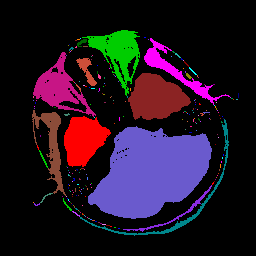
\includegraphics[scale=.7]{cthead1-label2-rgb}}
\subfigure[All the objects smaller than 1000 pixels removed]{\includegraphics[scale=.7]{cthead1-label2-size-bigger-than-1000}}
\subfigure[All the objects greater than 1000 pixels removed]{\includegraphics[scale=.7]{cthead1-label2-size-smaller-than-1000}}
\subfigure[All the objects with roundness smaller than 0.8 removed]{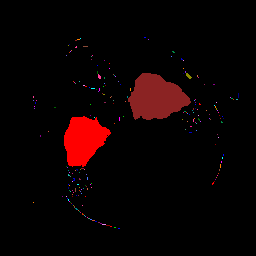
\includegraphics[scale=.7]{cthead1-label2-roundness-greater-than-0_8}}
\subfigure[All the objects with elongation smaller than 10 removed]{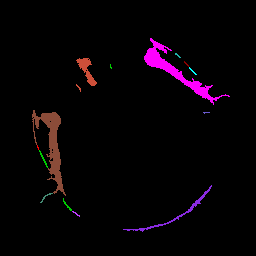
\includegraphics[scale=.7]{cthead1-label2-binaryElongation-greater-than-10}}
\subfigure[All the objects with perimeter smaller than 100 removed]{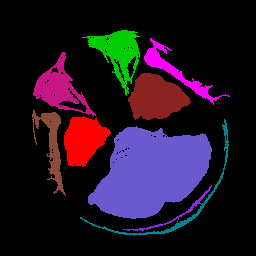
\includegraphics[scale=.7]{cthead1-label2-perimeter-greater-than-100}}
\caption{Some example of opening with different attribute and parameters.
Note that the labels are kept unchanged in the output image.}
\end{center}
\end{figure}


It can also be useful to simply get the attribute values associated with the
objects. In that case, the classes provided in with that article can be used in
place of {\em itk::LabelStatisticsImageFilter}, or to get some data about the
shape or the position of the object.

\subsection{Generating an itk::Image from the itk::LabelMap}

Once the manipulation of the objects is done, it can be useful to go back to a
more classic {\em itk::Image}. Several classes are provided to do that:
\begin{itemize}
  \item The {\em itk::LabelMapToLabelImageFilter} class simply
convert a {\em itk::LabelMap} to a label image stored in a {\em
itk::Image}.
  \item The {\em itk::LabelMapToBinaryImageFilter} put all the
objects in the foreground of a binary image stored in a {itk::Image}. It is
intended to be used with an image produced by the {\em
itk::BinaryImageToLabelMapFilter}. The background values of the
original image can also be restored by this filter.
  \item The {\em itk::LabelMapMaskImageFilter} class can be used
to mask an image with the objects of the {\em itk::LabelMap}. With
that filter, the image can be cropped to contain only the non-masked zone\footnote{
The code used to produce the output region based on the content of the image
is partially copied from a contribution of Peter Cech \url{http://www.vision.ee.ethz.ch/~pcech/itkAutoCropImageFilter/}.}
, or the non-masked zone padded by a user defined number of pixels.
  \item The {\em itk::LabelMapToAttributeImageFilter} produce
an {\em itk::Image} with the value of the attribute of the objects of the {\em
itk::LabelMap}. This filter is mostly useful to have a global view
of the attribute values in the image.
  \item The {\em LabelMapToRGBImageFilter} produce a color {\em itk::Image} with
{\em itk::RGBPixel} as pixel type. The label objects are in color, as in
Figure~\ref{fig:labelImage}. This class is mostly useful for a quick visual
validation without going outside ITK.
  \item Finally, the {\em LabelMapOvelayImageFilter} produce a color {\em itk::Image} with
{\em itk::RGBPixel} as pixel type. The label objects are in color on top of a grayscale
image, as in Figure~\ref{fig:nucleiOverlay}. This class is mostly useful for a quick visual
validation without going outside ITK.
\end{itemize}

\section{Prebuilt mini-pipeline filters}

The general view of the previous section show a very common way to use those
classes. To make them easier to use, some prebuilt classes have been made, to perform
the mini-pipeline:
\begin{itemize}
  \item creation of the {\em itk::LabelMap} from an {\em
itk::Image},
  \item valuation of the attribute(s) of the objects,
  \item filtering of the {\em itk::LabelMap},
  \item creation of an {\em itk::Image} from the filtered {\em
itk::LabelMap},
\end{itemize}
with a specific attribute.

Also, when using the {\em itk::ShapeLabelObject} or the {\em itk::StatisticsLabelObject}
class, we usually want them to be valuated. Some classes are provided to perform the
mini-pipeline:
\begin{itemize}
  \item creation of the {\em itk::LabelMap} from an {\em
itk::Image},
  \item valuation of the attributes of the objects
\end{itemize}
with the {\em itk::ShapeLabelObject} or the {\em itk::StatisticsLabelObject}.

Because the objects are often get from a label image or from a binary image,
those filters have been made for binary, and label images.

\subsection{Binary filters}

The filters to produce valuated attributes:

\begin{itemize}
  \item {\em itk::BinaryImageToShapeLabelMapFilter}
  \item {\em itk::BinaryImageToStatisticsLabelMapFilter}
\end{itemize}

The filters to fully hide the usage of the label objects:

\begin{itemize}
  \item {\em itk::BinaryAttributeKeepNObjectsImageFilter}
  \item {\em itk::BinaryAttributeOpeningImageFilter}
  \item {\em itk::BinaryShapeKeepNObjectsImageFilter}
  \item {\em itk::BinaryShapeOpeningImageFilter}
  \item {\em itk::BinaryStatisticsKeepNObjectsImageFilter}
  \item {\em itk::BinaryStatisticsOpeningImageFilter}
\end{itemize}

\subsection{Label filters}


The filters to produce valuated attributes:

\begin{itemize}
  \item {\em itk::LabelImageToShapeLabelMapFilter}
  \item {\em itk::LabelImageToStatisticsLabelMapFilter}
\end{itemize}

The filters to fully hide the usage of the label objects:

\begin{itemize}
  \item {\em itk::LabelAttributeKeepNObjectsImageFilter}
  \item {\em itk::LabelAttributeOpeningImageFilter}
  \item {\em itk::LabelShapeKeepNObjectsImageFilter}
  \item {\em itk::LabelShapeOpeningImageFilter}
  \item {\em itk::LabelStatisticsKeepNObjectsImageFilter}
  \item {\em itk::LabelStatisticsOpeningImageFilter}
  \item {\em itk::ShapeRelabelImageFilter}
  \item {\em itk::StatisticsRelabelImageFilter}
\end{itemize}

\section{Binary and label specialization of mathematical morphology filters}

All the following filters are using a morphological reconstruction, implemented internally
as an attribute opening with the {\em itk::AttributeLabelObject} class. Some binary filters
are implemented:

\begin{itemize}
  \item {\em itk::BinaryClosingByReconstructionImageFilter}
  \item {\em itk::BinaryFillholeImageFilter}
  \item {\em itk::BinaryGrindPeakImageFilter}
  \item {\em itk::BinaryOpeningByReconstructionImageFilter}
  \item {\em itk::BinaryReconstructionByDilationImageFilter}
  \item {\em itk::BinaryReconstructionByErosionImageFilter}
\end{itemize}

and some label filters, useful when the label objects are connected, or when we
want to avoid loosing the label by using a binary filter. Because the notion
of reconstruction by erosion is difficult with labels, only a few filters
are implemented:

\begin{itemize}
  \item {\em itk::LabelReconstructionByDilationImageFilter}
%  \item {\em itk::LabelOpeningByReconstructionImageFilter}
\end{itemize}


\section{Computation details}

\subsection{Binary image moments}

Central image moments for grayscale images are usually computed as

\begin{eqnarray}
Cm_{i,j} & = & \frac{S_{i,j}}{M} - Cg_i.Cg_j \\
S_{i,j}  & = & \sum_{p \in D} \left( I(p).p_i.p_j \right)
\end{eqnarray}

where $S_{i,j}$ is the central moment, $D$ is the domain of definition of the
image $I$, $I(p)$ is the pixel value of the image at the position $p$,
$0 \leq i < n$, $0 \leq i < n$, $n$ is the image dimension, $p_i$ is the
physical position on the axis $i$, $M$ is the total mass, $Cg$ is the center of
gravity. With binary images, $I(p)$ is either $0$ 
if $p$ is outside the object, or $1$ if $p$ is inside.

The complexity is $O(N_{P_I})$, where $N_{P_I}$ is the number of pixels in the image.


With the run-length encoding of the binary objects, the complexity can be decreased
to $O(N_{L_O})$, where $N_{L_O}$ is the number of lines in the object.

\begin{eqnarray}
S_{i,j} & = & \sum_{p \in D} \left( I(p).p_i.p_j \right) \\ \nonumber
         & = & \sum_{p \in O} \left( p_i.p_j \right) \\ \nonumber
         & = & \sum_{L \in O}  \sum_{p \in L} \left( p_i.p_j \right)
\end{eqnarray}

Where $O$ is a binary object in the image, and $L$ is a line of the object $O$, encoded
with the run-length encoding. In a line, $p_i$ is a constant if $i > 0$, so, $S_{i,j}$
can be written:

\begin{eqnarray}
S_{i,j} = \begin{cases}
  \underset{L \in O}\sum \left( l_L.p_i.p_j \right)                & \text{if $i > 0$ and $j > 0$}, \\
  \underset{L \in O}\sum \left( l_L.p_i.\underset{p \in L}\sum p_0 \right)  & \text{if $i > 0$ and $j = 0$}, \\
  \underset{L \in O}\sum \left( l_L.p_j.\underset{p \in L}\sum p_0 \right)  & \text{if $i = 0$ and $j > 0$}, \\
  \underset{L \in O}\sum \underset{p \in L}\sum p_0^2            & \text{if $i = j = 0$}.
           \end{cases}
\end{eqnarray}

It is known that
\begin{eqnarray}
\label{equ:sumx}
\sum_{x=0}^n x   & = & \frac{n(n+1)}{2} \\
\label{equ:sumx2}
\sum_{x=0}^n x^2 & = & \frac{n(n+1)(2n+1)}{6}
\end{eqnarray}

In order to use those formulae in the computation of $S_{i,j}$, the physical position has to be expanded in:
\begin{eqnarray}
\label{equ:expandedPosition}
p_j = o_j + s_j i_j
\end{eqnarray}
where $o_j$ is the origin of the line on the axis $j$, $s_j$ is the spacing on the axis $j$, and
$i_j$ is the index on the axis $j$.

With equations \ref{equ:expandedPosition}, \ref{equ:sumx} and \ref{equ:sumx2}, it is easy to remove the loop in the computation of the sum of physical positions of the axis $0$:

\begin{eqnarray}
\sum_{p \in L} p_0  & = & \sum_{i_0=0}^{l_L-1} (o_0 + s_0 i_0) \\ \nonumber
                    & = & l_L.o_0 + s_0\sum_{i_0=0}^{l_L-1} i_0 \\ \nonumber
                    & = & l_L.o_0 + s_0\left( \frac{(l_L-1)l_L}{2} \right) \\ \nonumber
                    & = & l_L \left( o_0 + \frac{s_0(l_L-1)}{2} \right)
\end{eqnarray}

where $l_L$ is the length of the line (in pixels), and in the sum of the square of the physical positions of the axis $0$:

\begin{eqnarray}
\sum_{p \in L} p_0^2  & = & \sum_{i_0=0}^{l_L-1} ( o_0 + s_0 i_0 )^2 \\ \nonumber
                      & = & \sum_{i_0=0}^{l_L-1} ( o_0^2 + s_0^2 i_0^2 + 2 o_0 i_0) \\ \nonumber
                      & = & l_L.o_0^2 + s_0^2\sum_{i_0=0}^{l_L-1} i_0^2 + 2 o_0 \sum_{i_0=0}^{l_L-1} i_0 \\ \nonumber
                      & = & l_L.o_0^2 + s_0^2 \left( \frac{(l_L-1)l_L(2l_L-1)}{6} \right) + 2 o_0 \left( \frac{(l_L-1)l_L}{2} \right) \\ \nonumber
                      & = & l_L\left( o_0^2 + (l_L-1)\left(\frac{s_0^2(2l_L-1)}{6}  + o_0 \right) \right)
\end{eqnarray}

Finally, $S_{i,j}$, used in the computation of the central moments, is computed as:
\begin{eqnarray}
S_{i,j} = \begin{cases}
  \underset{L \in O}\sum \left( l_L.p_i.p_j \right)                & \text{if $i > 0$ and $j > 0$}, \\
  \underset{L \in O}\sum \left( p_i.l_L^2 \left( o_0 + \frac{s_0(l_L-1)}{2} \right) \right) & \text{if $i > 0$ and $j = 0$}, \\
  \underset{L \in O}\sum \left( p_j.l_L^2 \left( o_0 + \frac{s_0(l_L-1)}{2} \right) \right) & \text{if $i = 0$ and $j > 0$}, \\
  \underset{L \in O}\sum \left( l_L\left( o_0^2 + (l_L-1)\left(\frac{s_0^2(2l_L-1)}{6}  + o_0 \right) \right) \right)            & \text{if $i = j = 0$}.
           \end{cases}
\end{eqnarray}


\subsection{Roundness}

The computation works with any image dimension, and so use the definition
of volume and area of an hypersphere in any dimension.

\begin{eqnarray}
\label{equ:hypersphereVolume}
V_n(r) = \frac{\pi^\frac{n}{2}r^n}{\Gamma(\frac{n}{2} + 1)}
\end{eqnarray}
where $V_n$ is the volume of the hypersphere $n$ is the image dimension,
and $r$ is the radius of the hypersphere.

\begin{eqnarray}
\Gamma\left(\frac{n}{2}+1\right) = \begin{cases}
  \left(\frac{n}{2}\right)!          & \text{if $n$ is even}, \\
  \sqrt{\pi}\frac{n!!}{2^{(n+1)/2}}  & \text{if $n$ is odd}.
                                   \end{cases}
\end{eqnarray}

$n!!$ is the {\em double factorial}, defined as:

\begin{eqnarray}
n!! = \begin{cases}
  1          & \text{if $n < 2$}, \\
  n (n-2)!!  & \text{if $n \geq 2$}.
      \end{cases}
\end{eqnarray}

\begin{eqnarray}
A_n(r) = {\frac{n V_n}{r}}
\end{eqnarray}

where $A_n$ is the area of the hypersphere.

\begin{eqnarray}
R = {\frac{A_n(r)}{a}}
\end{eqnarray}

where $R$ is the roundness, $a$ is the measured area of the 
object\footnote{More details about perimeter estimation will be published 
in another article.}, and the $r$ is the radius of an hypersphere with the
same volume than the object, computed using equation
\ref{equ:hypersphereVolume}.


\subsection{Pixel's neighborhood}

The run-length encoding does not allow an easy access to the neighbors of a
given pixel. If the neighborhood of all the pixels must be accessed, it is
much easier to convert the {itk::LabelMap} to a {\em itk::Image}
with the {\em itk::LabelMapToLabelImageFilter}, and use that
image to access the neighbors. That's what is done in {\em itk::ShapeLabelMapFilter}
to compute the maximum Feret diameter, and the perimeter estimation.

\section{Usage examples}

\subsection{Prebuilt pipelines}

\subsubsection{Binary shape opening}

The source code is available in the file {\em binary\_shape\_opening.cxx}.

\small \begin{verbatim}
#include "itkImageFileReader.h"
#include "itkImageFileWriter.h"
#include "itkSimpleFilterWatcher.h"

#include "itkBinaryShapeOpeningImageFilter.h"


int main(int argc, char * argv[])
{

  if( argc != 9 )
    {
    std::cerr << "usage: " << argv[0] << " input output foreground background lambda reverseOrdering connectivity attribute" << std::endl;
    // std::cerr << "  : " << std::endl;
    exit(1);
    }

  const int dim = 3;

  typedef itk::Image< unsigned char, dim > IType;

  typedef itk::ImageFileReader< IType > ReaderType;
  ReaderType::Pointer reader = ReaderType::New();
  reader->SetFileName( argv[1] );

  typedef itk::BinaryShapeOpeningImageFilter< IType > BinaryOpeningType;
  BinaryOpeningType::Pointer opening = BinaryOpeningType::New();
  opening->SetInput( reader->GetOutput() );
  opening->SetForegroundValue( atoi(argv[3]) );
  opening->SetBackgroundValue( atoi(argv[4]) );
  opening->SetLambda( atof(argv[5]) );
  opening->SetReverseOrdering( atoi(argv[6]) );
  opening->SetFullyConnected( atoi(argv[7]) );
  opening->SetAttribute( argv[8] );
  itk::SimpleFilterWatcher watcher(opening, "filter");

  typedef itk::ImageFileWriter< IType > WriterType;
  WriterType::Pointer writer = WriterType::New();
  writer->SetInput( opening->GetOutput() );
  writer->SetFileName( argv[2] );
  writer->Update();
  return 0;
}

\end{verbatim} \normalsize

\subsubsection{Statistics relabel}

The source code is available in the file {\em statistics\_relabel.cxx}.

\small \begin{verbatim}
#include "itkImageFileReader.h"
#include "itkImageFileWriter.h"
#include "itkSimpleFilterWatcher.h"

#include "itkStatisticsRelabelImageFilter.h"


int main(int argc, char * argv[])
{

  if( argc != 8 )
    {
    std::cerr << "usage: " << argv[0] << " input input output background useBg reverseOrdering attribute" << std::endl;
    // std::cerr << "  : " << std::endl;
    exit(1);
    }

  const int dim = 3;

  typedef itk::Image< unsigned char, dim > IType;

  typedef itk::ImageFileReader< IType > ReaderType;
  ReaderType::Pointer reader = ReaderType::New();
  reader->SetFileName( argv[1] );

  ReaderType::Pointer reader2 = ReaderType::New();
  reader2->SetFileName( argv[2] );

  typedef itk::StatisticsRelabelImageFilter< IType, IType > RelabelType;
  RelabelType::Pointer relabel = RelabelType::New();
  relabel->SetInput( reader->GetOutput() );
  relabel->SetFeatureImage( reader2->GetOutput() );
  relabel->SetBackgroundValue( atoi(argv[4]) );
  relabel->SetReverseOrdering( atoi(argv[6]) );
  relabel->SetAttribute( argv[7] );
  itk::SimpleFilterWatcher watcher(relabel, "filter");

  typedef itk::ImageFileWriter< IType > WriterType;
  WriterType::Pointer writer = WriterType::New();
  writer->SetInput( relabel->GetOutput() );
  writer->SetFileName( argv[3] );
  writer->Update();
  return 0;
}
\end{verbatim} \normalsize


\subsubsection{Label shape keep N obejcts}

The source code is available in the file {\em label\_shape\_keep\_n\_objects.cxx}.

\small \begin{verbatim}
#include "itkImageFileReader.h"
#include "itkImageFileWriter.h"
#include "itkSimpleFilterWatcher.h"

#include "itkLabelShapeKeepNObjectsImageFilter.h"


int main(int argc, char * argv[])
{

  if( argc != 7 )
    {
    std::cerr << "usage: " << argv[0] << " input output background nb reverseOrdering attribute" << std::endl;
    // std::cerr << "  : " << std::endl;
    exit(1);
    }

  const int dim = 3;

  typedef itk::Image< unsigned char, dim > IType;

  typedef itk::ImageFileReader< IType > ReaderType;
  ReaderType::Pointer reader = ReaderType::New();
  reader->SetFileName( argv[1] );

  typedef itk::LabelShapeKeepNObjectsImageFilter< IType > LabelOpeningType;
  LabelOpeningType::Pointer opening = LabelOpeningType::New();
  opening->SetInput( reader->GetOutput() );
  opening->SetBackgroundValue( atoi(argv[3]) );
  opening->SetNumberOfObjects( atoi(argv[4]) );
  opening->SetReverseOrdering( atoi(argv[5]) );
  opening->SetAttribute( argv[6] );
  itk::SimpleFilterWatcher watcher(opening, "filter");

  typedef itk::ImageFileWriter< IType > WriterType;
  WriterType::Pointer writer = WriterType::New();
  writer->SetInput( opening->GetOutput() );
  writer->SetFileName( argv[2] );
  writer->Update();
  return 0;
}
\end{verbatim} \normalsize

\subsubsection{Binary fill holes}

The source code is available in the file {\em binary\_fillhole.cxx}.

\small \begin{verbatim}
#include "itkImageFileReader.h"
#include "itkImageFileWriter.h"
#include "itkCommand.h"
#include "itkSimpleFilterWatcher.h"

#include "itkLabelObject.h"
#include "itkLabelMap.h"
#include "itkBinaryFillholeImageFilter.h"


int main(int argc, char * argv[])
{

  if( argc != 5 )
    {
    std::cerr << "usage: " << argv[0] << " input output conn fg" << std::endl;
    // std::cerr << "  : " << std::endl;
    exit(1);
    }

  const int dim = 2;

  typedef itk::Image< unsigned char, dim > IType;

  typedef itk::ImageFileReader< IType > ReaderType;
  ReaderType::Pointer reader = ReaderType::New();
  reader->SetFileName( argv[1] );
  reader->Update();

 typedef itk::BinaryFillholeImageFilter< IType > I2LType;
  I2LType::Pointer reconstruction = I2LType::New();
  reconstruction->SetInput( reader->GetOutput() );
  reconstruction->SetFullyConnected( atoi(argv[3]) );
  reconstruction->SetForegroundValue( atoi(argv[4]) );
//   reconstruction->SetBackgroundValue( atoi(argv[5]) );
  itk::SimpleFilterWatcher watcher(reconstruction, "filter");

  typedef itk::ImageFileWriter< IType > WriterType;
  WriterType::Pointer writer = WriterType::New();
  writer->SetInput( reconstruction->GetOutput() );
  writer->SetFileName( argv[2] );
  writer->Update();
  return 0;
}
\end{verbatim} \normalsize

\subsection{LabelObject and LabelMap manipulation}

% \subsubsection{LabelObject}
% 
% TODO
% 
% \subsubsection{ShapeLabelObject}
% 
% TODO
% 
% \subsubsection{StatisticsLabelObject}
% 
% TODO
% 
\subsubsection{AttributeLabelObject}

The {\em itk::AttributeLabelObject} let the user specify the type of the attribute
he wants to use, and thus is the good choice to implement a new attribute.

The source code is available in the file {\em generic\_attribute.cxx}.

First we include the headers of the class we will use, and parse the command line.

\small \begin{verbatim}
#include "itkImageFileReader.h"
#include "itkImageFileWriter.h"

#include "itkAttributeLabelObject.h"
#include "itkLabelMap.h"

#include "itkLabelImageToLabelMapFilter.h"

#include "itkAttributeKeepNObjectsLabelMapFilter.h"
#include "itkAttributeOpeningLabelMapFilter.h"
#include "itkAttributeRelabelLabelMapFilter.h"

#include "itkLabelMapToAttributeImageFilter.h"
#include "itkLabelMapToLabelImageFilter.h"


int main(int argc, char * argv[])
{

  if( argc != 10 )
    {
    std::cerr << "usage: " << argv[0] << " label input attr keep open relabel bg lambda nb" << std::endl;
    // std::cerr << "  : " << std::endl;
    exit(1);
    }
\end{verbatim} \normalsize
Declare the dimension used, and the type of the image for input and output.
\small \begin{verbatim}
  const int dim = 2;
  typedef unsigned char PType;
  typedef itk::Image< PType, dim > IType;
\end{verbatim} \normalsize
The AttributeLabelObject class take 3 template parameters: the 2 ones
from the LabelObject class, and the type of the attribute associated
with each node. Here we have chosen a double. We then declares the
type of the LabelMap with the type of the label object.
\small \begin{verbatim}
  typedef itk::AttributeLabelObject< unsigned long, dim, double > LabelObjectType;
  typedef itk::LabelMap< LabelObjectType > LabelMapType;
\end{verbatim} \normalsize
We read the input images.
\small \begin{verbatim}
  typedef itk::ImageFileReader< IType > ReaderType;
  ReaderType::Pointer reader = ReaderType::New();
  reader->SetFileName( argv[1] );

  ReaderType::Pointer reader2 = ReaderType::New();
  reader2->SetFileName( argv[2] );
\end{verbatim} \normalsize
And convert the label image to a LabelMap.
\small \begin{verbatim}
  typedef itk::LabelImageToLabelMapFilter< IType, LabelMapType > I2LType;
  I2LType::Pointer i2l = I2LType::New();
  i2l->SetInput( reader->GetOutput() );
  i2l->SetBackgroundValue( atoi(argv[7]) );
\end{verbatim} \normalsize
The next step is made outside the pipeline model, so we call Update() now.
\small \begin{verbatim}
  i2l->Update();
  reader2->Update();
\end{verbatim} \normalsize
Now we will valuate the attribute. The attribute will be the mean of the pixels
values in the 2nd image. Note that the StatisticsLabelObject can give us that value, without
having to code that by hand - that's an example.

Lets begin by declaring the iterator for the objects in the image, and get the object container, to reuse it later.
\small \begin{verbatim}
  LabelMapType::LabelObjectContainerType::const_iterator it;
  LabelMapType::Pointer labelMap = i2l->GetOutput();
  const LabelMapType::LabelObjectContainerType & labelObjectContainer = labelMap->GetLabelObjectContainer();
\end{verbatim} \normalsize
Now iterate over all the objects in the image.
\small \begin{verbatim}
  for( it = labelObjectContainer.begin(); it != labelObjectContainer.end(); it++ )
    {
\end{verbatim} \normalsize
The label is there if we need it, but it can also be found at labelObject->GetLabel().
\small \begin{verbatim}
    const PType & label = it->first;
    LabelObjectType * labelObject = it->second;
\end{verbatim} \normalsize
Init the variables used for the computation.
\small \begin{verbatim}
    double mean = 0;
    unsigned long size = 0;
\end{verbatim} \normalsize
Create the iterator for the lines, and iterate over them
\small \begin{verbatim}
    LabelObjectType::LineContainerType::const_iterator lit;
    LabelObjectType::LineContainerType lineContainer = labelObject->GetLineContainer();

    for( lit = lineContainer.begin(); lit != lineContainer.end(); lit++ )
      {
      const LabelMapType::IndexType & firstIdx = lit->GetIndex();
      const unsigned long & length = lit->GetLength();

      size += length;
\end{verbatim} \normalsize
Then iterate over all the pixels in the line, and get the pixel values in the feature image to compute their mean.
\small \begin{verbatim}
      long endIdx0 = firstIdx[0] + length;
      for( LabelMapType::IndexType idx = firstIdx; idx[0]<endIdx0; idx[0]++)
        {
        mean += reader2->GetOutput()->GetPixel( idx );
        }
      }
\end{verbatim} \normalsize
Complete the compuation of the mean, and set it as attibute value for the current object.
\small \begin{verbatim}
    mean /= size;
    labelObject->SetAttribute( mean );
\end{verbatim} \normalsize
The LabelObject class provides a Print() method to display its ivars.
\small \begin{verbatim}
    labelObject->Print( std::cout );

    }
\end{verbatim} \normalsize
Now that the objects have their attribute, we are free to manipulate them with
the common filters, or by hand. The default accessor (AttributeLabelObject)
is the wright one when using AttributeLabelObject so we don't have to specify it.
A different one can be used if needed though.
\small \begin{verbatim}
  typedef itk::AttributeKeepNObjectsLabelMapFilter< LabelMapType > KeepType;
  KeepType::Pointer keep = KeepType::New();
  keep->SetInput( labelMap );
  keep->SetReverseOrdering( true );
  keep->SetNumberOfObjects( atoi(argv[9]) );
\end{verbatim} \normalsize
Prevent the filter to run in place, so the input image is not modified.
\small \begin{verbatim}
  keep->SetInPlace( false );

  typedef itk::AttributeOpeningLabelMapFilter< LabelMapType > OpeningType;
  OpeningType::Pointer opening = OpeningType::New();
  opening->SetInput( labelMap );
  opening->SetLambda( atof(argv[8]) );
  opening->SetInPlace( false );

  typedef itk::AttributeRelabelLabelMapFilter< LabelMapType > RelabelType;
  RelabelType::Pointer relabel = RelabelType::New();
  relabel->SetInput( labelMap );
  relabel->SetInPlace( false );
\end{verbatim} \normalsize
The attribute values can be put directly in a classic image.
\small \begin{verbatim}
  typedef itk::LabelMapToAttributeImageFilter< LabelMapType, IType > A2IType;
  A2IType::Pointer a2i = A2IType::New();
  a2i->SetInput( labelMap );
\end{verbatim} \normalsize
Or the label collection can be converted back to an label image, or to a binary image
(not shown here)
\small \begin{verbatim}
  typedef itk::LabelMapToLabelImageFilter< LabelMapType, IType > L2IType;
  L2IType::Pointer l2i = L2IType::New();
\end{verbatim} \normalsize
Finally, write the results
\small \begin{verbatim}
  typedef itk::ImageFileWriter< IType > WriterType;
  WriterType::Pointer writer = WriterType::New();

  writer->SetInput( a2i->GetOutput() );
  writer->SetFileName( argv[3] );
  writer->Update();

  writer->SetInput( l2i->GetOutput() );

  l2i->SetInput( keep->GetOutput() );
  writer->SetFileName( argv[4] );
  writer->Update();

  l2i->SetInput( opening->GetOutput() );
  writer->SetFileName( argv[5] );
  writer->Update();

  l2i->SetInput( relabel->GetOutput() );
  writer->SetFileName( argv[6] );
  writer->Update();

  return 0;
}
\end{verbatim} \normalsize

\subsubsection{Custom attribute accessor}

This example shows how to use the LabelMap classes to remove all the
object with a bounding size smaller (or greater) than a given value
on the z axis.
The attribute we are interested is already computed by {\em ShapeLabelMapFilter}
and stored in {\em ShapeLabelObject}. It is not usable as is however, because it
is part of a multicomponent attribute: {\em Region}.

To be able to use it with the standard classes, we have to provide an accessor
which can be used by the opening filter.

The source code is available in the file {\em simple\_generic\_attribute.cxx}.

First include the classes we'll use
\small \begin{verbatim}
#include "itkImageFileReader.h"
#include "itkImageFileWriter.h"
#include "itkSimpleFilterWatcher.h"

#include "itkLabelImageToShapeLabelMapFilter.h"
#include "itkAttributeOpeningLabelMapFilter.h"
#include "itkLabelMapToLabelImageFilter.h"
\end{verbatim} \normalsize
Now we can declare the custom accessor type, which will be used by the opening
filter.
\small \begin{verbatim}
template< class TLabelObject >
class ITK_EXPORT LastDimesionRegionSizeObjectAccessor
{
public:
\end{verbatim} \normalsize
The declaration of {\em AttributeValueType} is mandatory. It is used internally
in the opening filter to define the type of the lambda value.
{\em AttributeValueType} should be the same as the type returned by the operator()
method.
\small \begin{verbatim}
  typedef unsigned long AttributeValueType;
\end{verbatim} \normalsize
{\em operator()} is the core of the accessor. It takes a label object as parameter,
and return the attribute of interest. Some computations can be done inside the accessor
method, but they should be as fast as possible, because {\em operator()} may be called
many time by some filters. If an attribute value takes time to compute, it should rather be computed once
for all and stored in a new attribute. In that case, there is no computation at all, only
an access to a value hidden in a multicomponent attribute, so things are very fast.
\small \begin{verbatim}
  inline const AttributeValueType operator()( const TLabelObject * labelObject )
    {
    return labelObject->GetRegion().GetSize()[TLabelObject::ImageDimension-1];
    }
};
\end{verbatim} \normalsize
Now the main program. First the usual validation of the number of arguments.
\small \begin{verbatim}
int main(int argc, char * argv[])
{

  if( argc != 6 )
    {
    std::cerr << "usage: " << argv[0] << " input output bg lambda reverse" << std::endl;
    // std::cerr << "  : " << std::endl;
    exit(1);
    }
\end{verbatim} \normalsize
Let's declare the dimension used, and the type of the input image
\small \begin{verbatim}
  const int dim = 3;
  typedef unsigned char PType;
  typedef itk::Image< PType, dim > IType;
\end{verbatim} \normalsize
We read the input image.
\small \begin{verbatim}
  typedef itk::ImageFileReader< IType > ReaderType;
  ReaderType::Pointer reader = ReaderType::New();
  reader->SetFileName( argv[1] );
\end{verbatim} \normalsize
And convert it to a {\em LabelMap}, with the shape attributes computed.
We use the default label object type provided by {\em LabelImageToShapeLabelMapFilter}.
\small \begin{verbatim}
  typedef itk::LabelImageToShapeLabelMapFilter< IType > I2LType;
  I2LType::Pointer i2l = I2LType::New();
  i2l->SetInput( reader->GetOutput() );
  i2l->SetBackgroundValue( atoi(argv[3]) );
\end{verbatim} \normalsize
The opening filter is declared with our custom accessor type as second
template argument, so it will be able to user our custom attribute to make
the opening.
\small \begin{verbatim}
  typedef LastDimesionRegionSizeObjectAccessor< I2LType::LabelObjectType > AccessorType;
  typedef itk::AttributeOpeningLabelMapFilter< I2LType::OutputImageType, AccessorType > OpeningType;
  OpeningType::Pointer opening = OpeningType::New();
  opening->SetInput( i2l->GetOutput() );
  opening->SetLambda( atof(argv[4]) );
  opening->SetReverseOrdering( atof(argv[5]) );
  itk::SimpleFilterWatcher watcher(opening, "filter");
\end{verbatim} \normalsize
The label map is then converted back to an label image.
\small \begin{verbatim}
  typedef itk::LabelMapToLabelImageFilter< I2LType::OutputImageType, IType > L2IType;
  L2IType::Pointer l2i = L2IType::New();
  l2i->SetInput( opening->GetOutput() );
\end{verbatim} \normalsize
Write the result to the disk.
\small \begin{verbatim}
  typedef itk::ImageFileWriter< IType > WriterType;
  WriterType::Pointer writer = WriterType::New();
  writer->SetInput( l2i->GetOutput() );
  writer->SetFileName( argv[2] );
  writer->Update();
\end{verbatim} \normalsize
Finally, print all the label objects after the opening, to check everything has been done right.
\small \begin{verbatim}
  opening->GetOutput()->PrintLabelObjects();
  std::cout << "Number of objects after the opening: " << opening->GetOutput()->GetNumberOfLabelObjects() << std::endl;
  
  return 0;
}
\end{verbatim} \normalsize


\subsection{Reading attribute values}

In that example, we will read a binary image, and get some of attributes
about the obejcts contained in that image.
The source code is available in the file {\em attribute\_values.cxx}.

First include the classes we'll use
\small \begin{verbatim}
#include "itkImageFileReader.h"
#include "itkShapeLabelObject.h"
#include "itkLabelMap.h"
#include "itkBinaryImageToLabelMapFilter.h"
#include "itkShapeLabelMapFilter.h"

int main(int, char * argv[])
{
  const int dim = 2;
\end{verbatim} \normalsize
then declare the type of the input image
\small \begin{verbatim}
  typedef unsigned char PixelType;
  typedef itk::Image< PixelType, dim >    ImageType;
  
\end{verbatim} \normalsize
read the input image
\small \begin{verbatim}
  typedef itk::ImageFileReader< ImageType > ReaderType;
  ReaderType::Pointer reader = ReaderType::New();
  reader->SetFileName( argv[1] );
  
\end{verbatim} \normalsize
define the object type. Here the ShapeLabelObject type
is chosen in order to read some attribute related to the shape
of the objects (by opposition to the content of the object, with
the StatisticsLabelObejct).
\small \begin{verbatim}
  typedef unsigned long LabelType;
  typedef itk::ShapeLabelObject< LabelType, dim > LabelObjectType;
  typedef itk::LabelMap< LabelObjectType > LabelMapType;

\end{verbatim} \normalsize
convert the image in a collection of objects
\small \begin{verbatim}
  typedef itk::BinaryImageToLabelMapFilter< ImageType, LabelMapType > ConverterType;
  ConverterType::Pointer converter = ConverterType::New();
  converter->SetInput( reader->GetOutput() );
  converter->SetForegroundValue( 200 );

\end{verbatim} \normalsize
and valuate the attributes with the dedicated filter: ShapeLabelMapFilter
\small \begin{verbatim}
  typedef itk::ShapeLabelMapFilter< LabelMapType > ShapeFilterType;
  ShapeFilterType::Pointer shape = ShapeFilterType::New();
  shape->SetInput( converter->GetOutput() );

\end{verbatim} \normalsize
update the shape filter, so its output will be up to date
\small \begin{verbatim}
  shape->Update();

\end{verbatim} \normalsize
then we can read the attribute values we're interested in. {\em itk::BinaryImageToLabelMapFilter}
produces consecutives labels, so a simple {for} loop will do the job.
\small \begin{verbatim}
  LabelMapType::Pointer labelMap = converter->GetOutput();
  for( unsigned int label=1; label<=labelMap->GetNumberOfLabelObjects(); label++ )
    {
    // we don't need a SmartPointer of the label object here, because the reference is kept in
    // in the label map.
    const LabelObjectType * labelObject = labelMap->GetLabelObject( label );
    std::cout << label << "\t" << labelObject->GetPhysicalSize() << "\t" << labelObject->GetCentroid() << std::endl;
    }
  
  return 0;
}
\end{verbatim} \normalsize


\subsection{The mask features}

The {\em itk::LabelMapMaskImageFilter} class let the user mask
a part of an {\em itk::Image} with the objects of a {\em itk::LabelMap}.
It can also crop the image to contain only the masked region.

The source code is available in the file {\em mask.cxx}.

First we include the headers of the class we will use, and parse the command line.

\small \begin{verbatim}
#include "itkImageFileReader.h"
#include "itkImageFileWriter.h"
#include "itkSimpleFilterWatcher.h"

#include "itkLabelObject.h"
#include "itkLabelMap.h"
#include "itkLabelImageToLabelMapFilter.h"
#include "itkLabelMapMaskImageFilter.h"


int main(int argc, char * argv[])
{

  if( argc != 9 )
    {
    std::cerr << "usage: " << argv[0] << " labelImage input output label bg neg crop cropBorder" << std::endl;
    // std::cerr << "  : " << std::endl;
    exit(1);
    }
\end{verbatim} \normalsize
the filters are able to work in any dimension. Lets choose 3, so the program can be tested on
2D and 2D image.
\small \begin{verbatim}
  const int dim = 3;
\end{verbatim} \normalsize
declare the input image type
\small \begin{verbatim}
  typedef itk::Image< unsigned char, dim > ImageType;
\end{verbatim} \normalsize
and the label object type to use. The input image is a label image, so the 
type of the label can be the same type than the pixel type. itk::LabelObject is
chosen, because only the mask feature is tested here, so we don't need any
attribute.
\small \begin{verbatim}
  typedef itk::LabelObject< unsigned char, dim > LabelObjectType;
  typedef itk::LabelMap< LabelObjectType > LabelMapType;
\end{verbatim} \normalsize
read the label image and the input image to be masked.
\small \begin{verbatim}
  typedef itk::ImageFileReader< ImageType > ReaderType;
  ReaderType::Pointer reader = ReaderType::New();
  reader->SetFileName( argv[1] );
  
  ReaderType::Pointer reader2 = ReaderType::New();
  reader2->SetFileName( argv[2] );
\end{verbatim} \normalsize
convert the label image to a label collection image.
\small \begin{verbatim}
  typedef itk::LabelImageToLabelMapFilter< ImageType, LabelMapType> I2LType;
  I2LType::Pointer i2l = I2LType::New();
  i2l->SetInput( reader->GetOutput() );
\end{verbatim} \normalsize
then mask the image. Two inputs are required (the label collection image, and
the image to be masked). The label used to mask the image is passed with the 
{\em SetLabel()} method. The background in the output image, where the image is masked,
is passed with {\em SetBackground()}. The user can choose to mask the image outside the
label object (that's the default behavior), or inside the label object with the
chosen label, by calling {\em SetNegated()}. Finally, the image can be cropped to the
masked region, by calling {\em SetCrop(true)}, or to a region padded by a border, by
calling both {\em SetCrop()} and {\em SetCropBorder()}. The crop border defaults to $0$, and the
image is not cropped by default.
\small \begin{verbatim}
  typedef itk::LabelMapMaskImageFilter< LabelMapType, ImageType > MaskType;
  MaskType::Pointer mask = MaskType::New();
  mask->SetInput( i2l->GetOutput() );
  mask->SetFeatureImage( reader2->GetOutput() );
  mask->SetLabel( atoi(argv[4]) );
  mask->SetBackgroundValue( atoi(argv[5]) );
  mask->SetNegated( atoi(argv[6]) );
  mask->SetCrop( atoi(argv[7]) );
  MaskType::SizeType border;
  border.Fill( atoi(argv[8]) );
  mask->SetCropBorder( border );
  itk::SimpleFilterWatcher watcher6(mask, "filter");
\end{verbatim} \normalsize
Finally, save the output image.
\small \begin{verbatim}
  typedef itk::ImageFileWriter< ImageType > WriterType;
  WriterType::Pointer writer = WriterType::New();
  writer->SetInput( mask->GetOutput() );
  writer->SetFileName( argv[3] );
  writer->Update();

  return 0;
}
\end{verbatim} \normalsize



\subsection{A full python example}

In that example, we want to:
\begin{itemize}
\item find the nuclei in the first image
\item find the spots insice the nucleus in the second image
\item get the mean value in the nucleus, in the zone of each spot.
\end{itemize}

\begin{figure}[htbp]
\begin{center}
\subfigure[Nucleus]{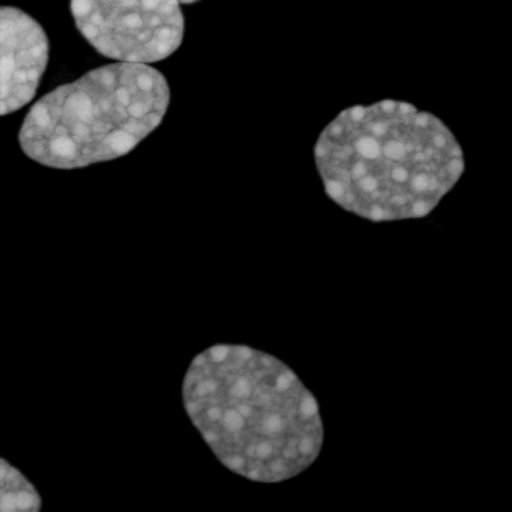
\includegraphics[scale=0.45]{noyaux}}
\subfigure[Spots]{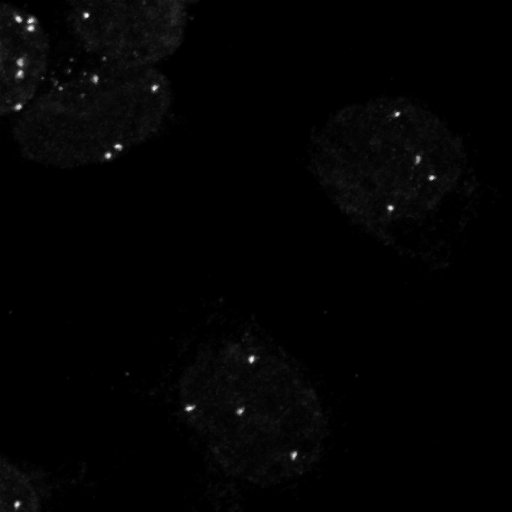
\includegraphics[scale=0.45]{spots}}
\caption{The input images.}
\end{center}
\end{figure}


The source code is available in example.py.

Lets begin with the usual {\em import}s.
\small \begin{verbatim}
import itk, sys
itk.auto_progress()
\end{verbatim} \normalsize
Then declare the type we will use, as is {\em c++}.
\small \begin{verbatim}
Dimension = 2
PixelType = itk.UC
ImageType = itk.Image[ PixelType, Dimension ]

DistancePixelType = itk.F
DistanceImageType = itk.Image[ DistancePixelType, Dimension ]

RGBPixelType = itk.RGBPixel[PixelType]
RGBImageType = itk.Image[ RGBPixelType, Dimension ]

LabelObjectType = itk.StatisticsLabelObject[itk.UL, Dimension]
LabelMapType = itk.LabelMap[LabelObjectType]
\end{verbatim} \normalsize
read the image of the nucleus
\small \begin{verbatim}
nuclei = itk.ImageFileReader[ImageType].New(FileName="images/noyaux.png")
\end{verbatim} \normalsize
perform a simple binarization. Note that the Otsu filter does not use the same convention as usual: the white part is outside.
\small \begin{verbatim}
otsu = itk.OtsuThresholdImageFilter[ImageType, ImageType].New(nuclei, OutsideValue=255,
    InsideValue=0)
\end{verbatim} \normalsize
The nuclei are not separated. We split them with a watershed.
\small \begin{verbatim}
maurer = itk.SignedMaurerDistanceMapImageFilter[ImageType, DistanceImageType].New(otsu)
watershed = itk.MorphologicalWatershedImageFilter[DistanceImageType, ImageType].New(maurer,
    Level=60, MarkWatershedLine=False)
mask = itk.MaskImageFilter[ImageType, ImageType, ImageType].New(watershed, otsu)
\end{verbatim} \normalsize
And now switch to the label collection representation
\small \begin{verbatim}
label = itk.LabelImageToLabelMapFilter[ImageType, LabelMapType].New(mask)
\end{verbatim} \normalsize
compute the attribute values
\small \begin{verbatim}
stats = itk.StatisticsLabelMapFilter[LabelMapType, ImageType].New(label, nuclei)
\end{verbatim} \normalsize
drop the objects too small to be a nucleus, and the ones on the border
\small \begin{verbatim}
size = itk.ShapeOpeningLabelMapFilter[LabelMapType].New(stats,Attribute='Size',
    Lambda=100)
border = itk.ShapeOpeningLabelMapFilter[LabelMapType].New(size, Attribute='SizeOnBorder',
    Lambda=10, ReverseOrdering=True)
\end{verbatim} \normalsize
Reoder the labels. The objects with the highest mean are the first ones.
\small \begin{verbatim}
relabel = itk.StatisticsRelabelLabelMapFilter[LabelMapType].New(border, Attribute='Mean')
\end{verbatim} \normalsize
for visual validation:
\small \begin{verbatim}
labelNuclei = itk.LabelMapToLabelImageFilter[LabelMapType, ImageType].New(relabel)
overlay = itk.LabelOverlayImageFilter[ImageType, ImageType, RGBImageType].New(nuclei,
    labelNuclei, UseBackground=True)
itk.write(overlay, "nuclei-overlay.png")
\end{verbatim} \normalsize

\begin{figure}
\begin{center}
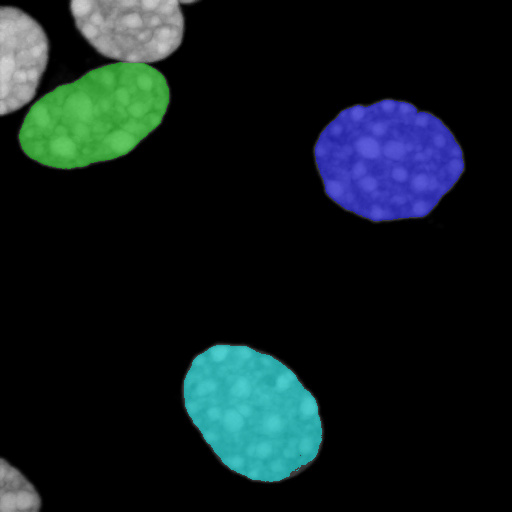
\includegraphics[scale=0.45]{nuclei-overlay}
\caption{The segmented nuclei. The too small objects and the ones on the border have been excluded.}
\label{fig:nucleiOverlay}
\end{center}
\end{figure}

Now, the spots:
\small \begin{verbatim}
spots = itk.ImageFileReader[ImageType].New(FileName="images/spots.png")
\end{verbatim} \normalsize
Mask the spot image to keep only the nucleus zone. The rest of the image is cropped, excepted a border of 2 pixels
\small \begin{verbatim}
maskSpots = itk.LabelMapMaskImageFilter[LabelMapType, ImageType].New(relabel, spots, Label=1,
    Crop=True, CropBorder=2)
\end{verbatim} \normalsize
A simple thresholding:
\small \begin{verbatim}
th = itk.BinaryThresholdImageFilter[ImageType, ImageType].New(maskSpots, LowerThreshold=110)
\end{verbatim} \normalsize
Now swith to the label collection representation, and compute the attribute values. This time, the input image is not a label image, but a binary one.
\small \begin{verbatim}
slabel = itk.BinaryImageToLabelMapFilter[ImageType, LabelMapType].New(th)
sstats = itk.StatisticsLabelMapFilter[LabelMapType, ImageType].New(slabel, nuclei)
\end{verbatim} \normalsize
we know there are for spots in the nubleus, so keep the 4 biggest spots. The other attribute are also usable - we may have chosen to keep the 4 brightest spots for example.
\small \begin{verbatim}
skeep = itk.ShapeKeepNObjectsLabelMapFilter[LabelMapType].New(sstats, Attribute='Size',
    NumberOfObjects=4)
\end{verbatim} \normalsize
Reoder the labels. The bigger objects first.
\small \begin{verbatim}
srelabel = itk.StatisticsRelabelLabelMapFilter[LabelMapType].New(skeep, Attribute='Size')
\end{verbatim} \normalsize
Finally, display the values we are interested in:
\begin{itemize}
  \item the nucleus number,
  \item the spot position,
  \item the mean value in the nucleus in the spot zone.
\end{itemize}

\small \begin{verbatim}
print "nuclei", "x", "y", "mean"

for nl in range(1, relabel.GetOutput().GetNumberOfLabelObjects()+1):
  maskSpots.SetLabel(nl)
  srelabel.UpdateLargestPossibleRegion()
  labeCollection = srelabel.GetOutput()

  for l in range(1, labeCollection.GetNumberOfLabelObjects()+1):
    lo = labeCollection.GetLabelObject(l)
    print nl, lo.GetCentroid()[0], lo.GetCentroid()[1], lo.GetMean()
\end{verbatim} \normalsize


\begin{table}[phtb]
\centering
\small
\begin{tabular}{cccc}
\hline
nucleus	& x	& y	& mean	\\
\hline
1	& 117.925925926	& 146.111111111	& 188.185185185	\\
1	& 154.25	& 87.4166666667	& 126.416666667	\\
1	& 107.666666667	& 155.125	& 122.0	\\
1	& 95.2380952381	& 78.2857142857	& 121.0	\\
2	& 417.631578947	& 158.736842105	& 132.894736842	\\
2	& 431.277777778	& 177.388888889	& 131.222222222	\\
2	& 390.117647059	& 207.588235294	& 96.8235294118	\\
2	& 396.8		& 113.666666667	& 113.2	\\
3	& 251.148148148	& 358.814814815	& 105.037037037	\\
3	& 189.333333333	& 407.888888889	& 111.074074074	\\
3	& 293.72	& 454.8		& 95.48	\\
3	& 239.888888889	& 411.111111111	& 135.222222222	\\
\hline
\hline
\end{tabular}
\caption{Output of the python example.}
\end{table}


\section{Threading support}

When possible, the filters provided with that contribution have been multithreaded.
Some of them however, are not (easily) threadable (the {\em KeepNObjects} and {\em Relabel}
filters), or shouldn't get any performance improvement in a threaded version
(the {\em Opening} filters).

The {\em itk::BinaryImageToLabelMapFilter} class is a slight modification of the
Richard Beare's {\em itk::ConnectedComponentImageFilter}, and have also been threaded
to get the best of the performances on a multicore system.

The classical thread architecture is used when the input image is an {\em itk::Image}: the image
is splitted in several regions (one per thread), and each thread work on its own region.

Because the {\em itk::LabelMap} image is not an array of pixels, it can't be splitted
that way. Instead, several threads are created, and try to take an object in the collection.
If they get one, they process that object individually, and try to get another one when the
object is processed. If no object can be get, the thread ends. A {\em itk::FastMutexLock} is used
to ensure that only one thread take an object at a time.

For the developer, the usage of the threading support is made very simple, by subclassing
{\em itk::LabelMapFilter}, or {\em itk::InPlaceLabelMapFilter}, and implementing
the method {\em virtual void ThreadedGenerateData( LabelObjectType * labelObject )} in the
new class. This method only has to process the labelObject passed in parameter. All the
threading code and mutex lock management is already implemented. The mutex lock remain
accessible if the subclass need to use it, as the {\em m\_LabelObjectContainerLock} ivar.

\section{In place filtering}

All the filters which are taking a {\em itk::LabelMap} as input, and are producing a {\em itk::LabelMap} as output, are implemented as a subclass of {\em InPlaceLabelMapFilter} and
thus are running in place by default.

The use can modify this behavior with the {\em SetInPlace( bool )}, {\em InPlaceOn()}, and {\em InPlaceOff()} methods, as with the usual {\em InPlaceImageFilter}.

To use that feature, a developer only have to subclass {\em InPlaceLabelMapFilter} and
implement the {\em virtual void ThreadedGenerateData( LabelObjectType * labelObject )}, to get easy thread
support \footnote{see the previous section}, or the {\em virtual void GenerateData()} if the filter is not threadable. In that last case,
the only image to manipulate is the one get with the {\em GetOutput()} method, which is the input image if the filter runs in place, or a copy of the input image if the filter is not running in place.


\section{Wrappers support}

All the classes provided with that article, excepted the most generic ones made
to help the developer to implement some new features, can be used with both stable and unstable WrapITK,
and have been fully tested with python.

% \section{Performance}
% 
% TODO

\section{Known bugs and future work}

To fit the ITK style, some iterators should be implemented to be able to iterate
over all the 
\begin{itemize}
  \item objects,
  \item lines,
  \item or pixels
\end{itemize}

of an image, starting from 
\begin{itemize}
  \item an image,
  \item an object,
  \item or a line.
\end{itemize}

Doing that require a good knowledge of the iterator design. Any help on that point is
welcome.

It may be useful to implement the most commonly used opening, keep N objects and relabel transforms in a more efficient way, by using an {\em itk::AttributeLabelObject} instead of a {\em itk::ShapeLabelObject} or a {\em itk::StatisticsLabelObject}.

The {\em itk::BinaryImageToLabelMapFilter} class should be threaded to get the best of that filter on multiprocessors systems.

The converters from/to image are provided, but it may be useful to  have the converters from/to other objects representations:
\begin{itemize}
  \item spatial objects,
  \item meshs,
  \item structuring elements.
\end{itemize}


Finally, all the binary and label filters should be implemented as a subclass of {\em itk::InPlaceImageFilter}.

Note that some names have been changed in revision 3. To fix your sources, the following commands can be used in your source directory (order is important):
\small \begin{verbatim}
perl -e 's/LabelCollectionImage/LabelMap/g' -pi *
perl -e 's/GetNumberOfObjects/GetNumberOfLabelObjects/g' -pi *
perl -e 's/PrintObjects/PrintLabelObjects/g' -pi *
perl -e 's/LabelMapToMaskImageFilter/LabelMapMaskImageFilter/g' -pi *
\end{verbatim} \normalsize

\section{Conclusion}

ITK is currently lacking a good way to manipulate the binary objects. With that contribution I hope to have mostly
filled that lack.

\section{Acknowledgments}
I thank Richard Beare for his suggestion to use the run length encoding to represent the binary objects, and Julien Jomier for his help for the choice to {\em not} use the {\em itk::SpatialObject} class as base class of the {\em itk::LabelObject} class.

I thank Dr Pierre Adenot and MIMA2 confocal facilities
(\url{http://mima2.jouy.inra.fr}) for providing the 3D test image.
% I am grateful to the INRA MIGALE bioinformatics platform
% (\url{http://migale.jouy.inra.fr}) for providing the computational resources
% used for the timing tests.
I thank Dr Maria Ballester for providing the image used in the python example.


\appendix



\bibliographystyle{plain}
\bibliography{InsightJournal}
\nocite{ITKSoftwareGuide}

\end{document}

